\chapter{Results}

\section{Introduction}
%introduce the results section and what processing will be done
The information gathered from the previous section is used to estimate the azimuth and elevation angles of the transmitter. First the azimuth angle will be estimated which will provide the information necessary for calculating the elevation angle. 

%-----------------------------------------------------------------------------------------------------------------------------------------------------------------------

\section{Transmitter Azimuth Angle Estimation}
%formulate the estimation equation and discuss ambiguity considerations
The azimuth angle estimation technique is based on the data collected by rotating the helicopter platform in a clockwise manner, during which at a set angle a doppler envelope is calculated and subsequent maximum and minimum values are collected. After a complete rotation the doppler maximum and minimum values produce a sinusoidal pattern as shown in figure \ref{fig:tx_azimuth_angle_200} without the assumption of knowing the starting azimuth angle. With this data we need to find an unambiguous angle that will set the coordinate space and provide an estimate of current azimuth angle. To do this the absolute value of the minimum envelope data is superimposed onto the maximum envelope data as shown in figure \ref{fig:azimuth_estimation_max_vs_absMin}.

\begin{figure}
	\begin{center}
		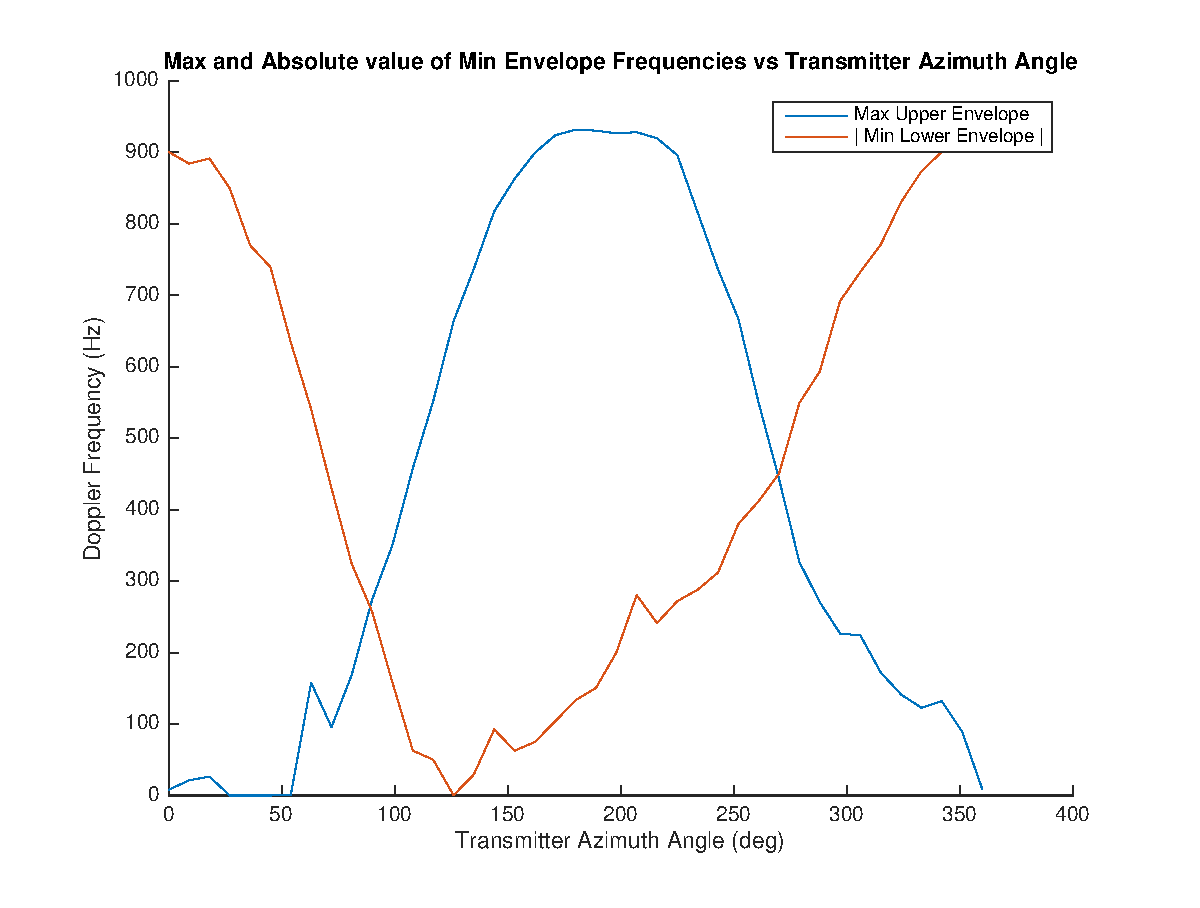
\includegraphics[width=10cm]{images/results/Azimuth_angle_estimation_max_vs_absMin.eps}
		\caption{Max and Absolute value of Min Envelope Frequencies vs Transmitter Azimuth Angle at an Elevation Angle of 45\textdegree}
		\label{fig:azimuth_estimation_max_vs_absMin}
	\end{center}
\end{figure}

From figure \ref{fig:azimuth_estimation_max_vs_absMin} there are two points at which the maximums and the absolute value of the minimums cross. By computing the difference \ref{eqn:difference}

%formula for difference
\begin{equation}
	 Envelope Difference = Max Upper Envelope - | Min Lower Envelope |
	 \label{eqn:difference}
\end{equation}

we produce an almost exact sinusoid centered around zero, shown in figure \ref{fig:azimuth_estimation_difference}.

 \begin{figure}
	\begin{center}
		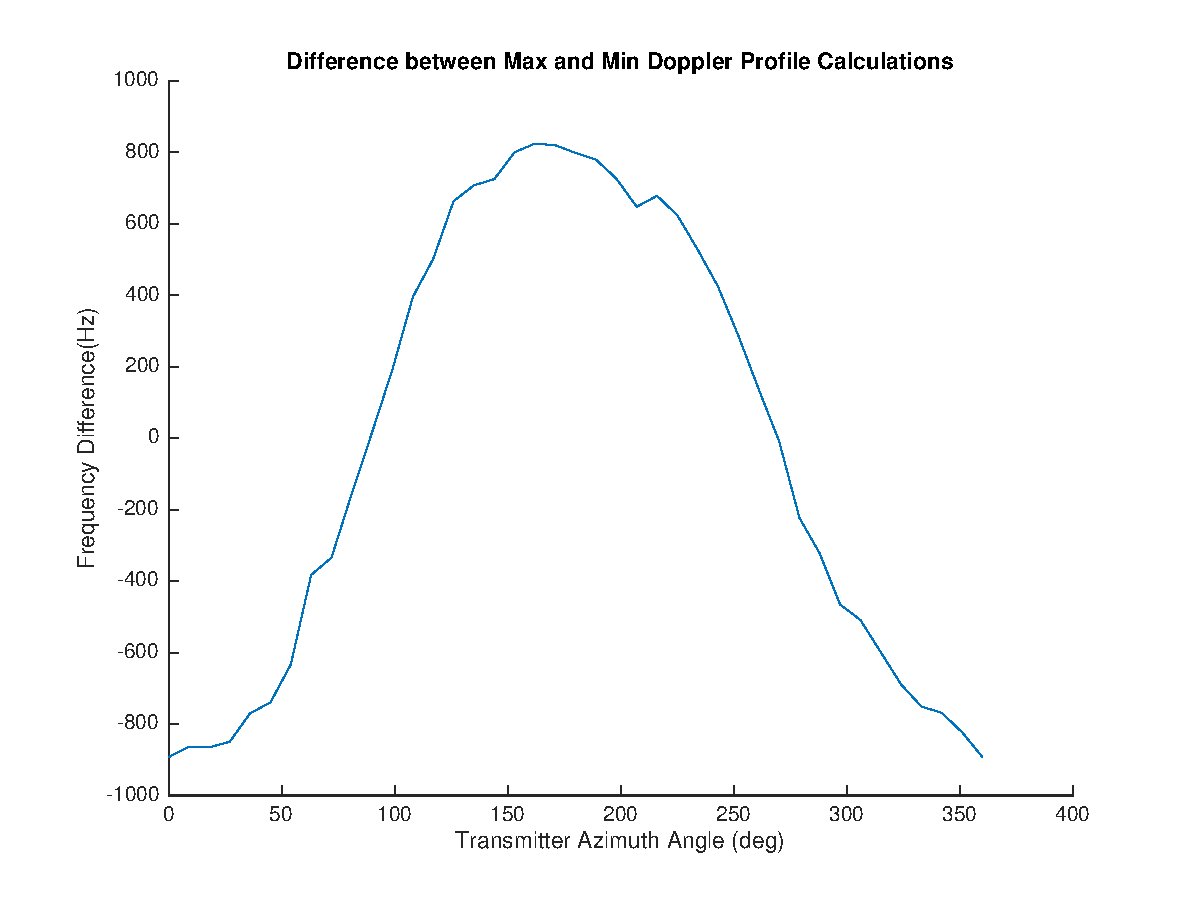
\includegraphics[width=10cm]{images/results/Azimuth_angle_estimation_difference.eps}
		\caption{Difference between Max and Min Envelope Calculations vs Transmitter Azimuth Angle at an Elevation Angle of 45\textdegree}
		\label{fig:azimuth_estimation_difference}
	\end{center}
\end{figure}

While figure \ref{fig:azimuth_estimation_difference} provides information about the angle of the transmitter it does not contain enough to locate an unambiguous azimuth angle in itself, therefore by computing \ref{eqn:addition}

% -------------------------dont use------------------------------------
%formula for addition
\begin{equation}
	 Envelope Addition = Max Upper Envelope + | Min Lower Envelope |
	 \label{eqn:addition}
\end{equation}

it results in a trend that contains a global minimum at an azimuth of 90\textdegree \space as shown in figure \ref{fig:azimuth_estimation_max_plus_absMin}. 

 \begin{figure}
	\begin{center}
		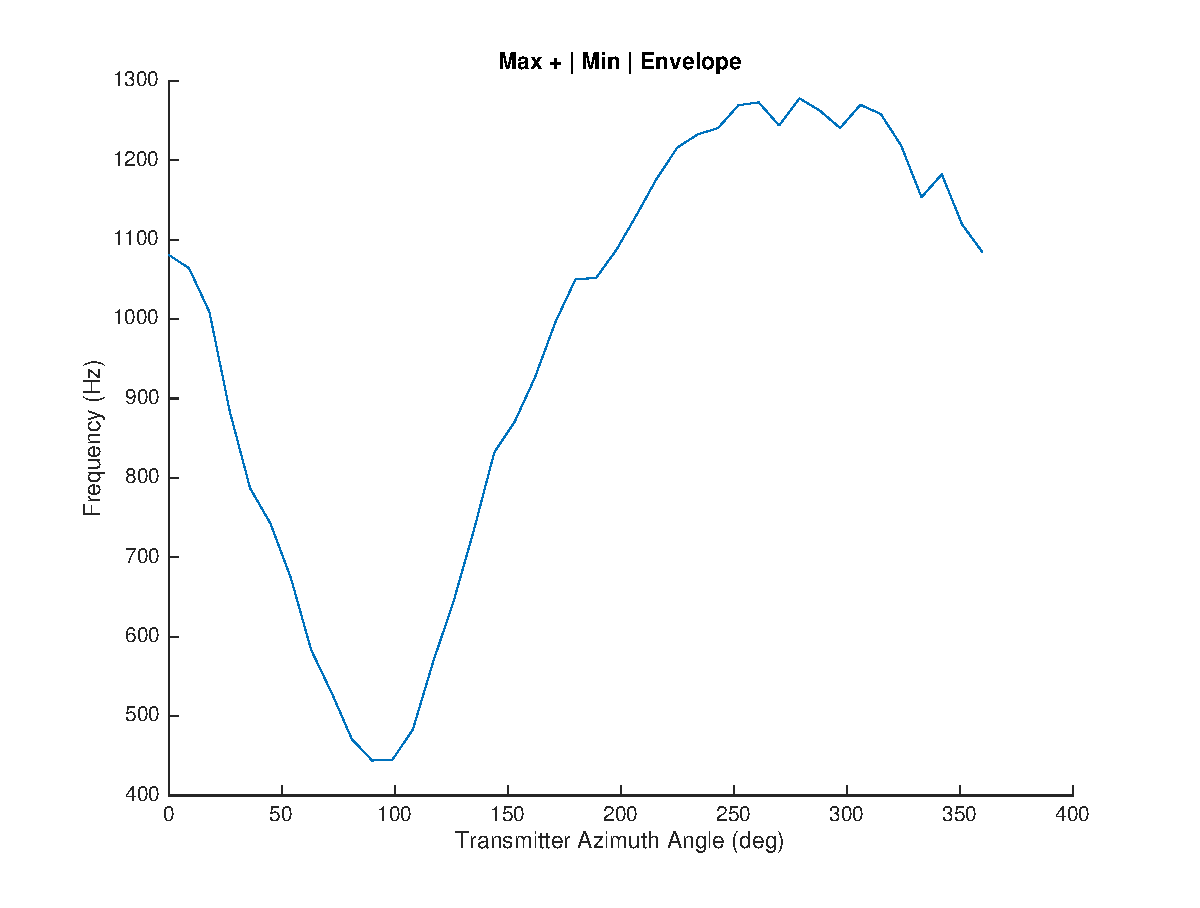
\includegraphics[width=10cm]{images/results/Azimuth_angle_estimation_max_plus_absMin.eps}
		\caption{Max plus Absolute value of Min envelope Frequencies vs Transmitter Azimuth Angle at an Elevation Angle of 45\textdegree}
		\label{fig:azimuth_estimation_max_plus_absMin}
	\end{center}
\end{figure}
% -------------------------dont use------------------------------------

Finding the index location of the minimum determines the point at which the transmitter is at an azimuth of 90\textdegree. Which means the transmitter and receiver are in line with each other producing the case from model \ref{fig:3D_model_90az}. The 90\textdegree \space location is displayed in figure \ref{fig:azimuth_estimation_plotted} which places the point on the difference between max and min envelopes therefore providing an accurate representation of the transmitters azimuth angle.

  \begin{figure}
	\begin{center}
		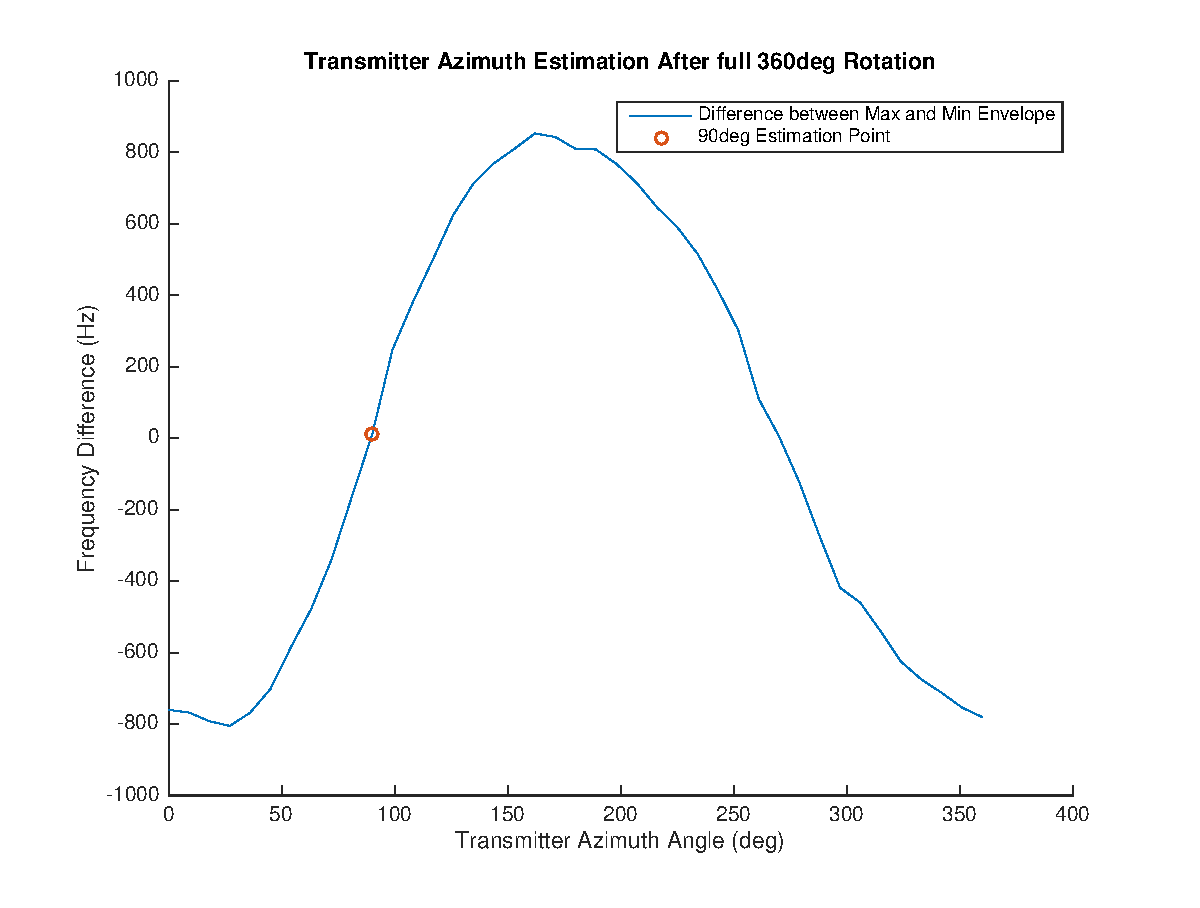
\includegraphics[width=10cm]{images/results/Azimuth_angle_estimation_plotted.eps}
		\caption{Transmitter Azimuth Estimation After full 360deg Rotation at an Elevation Angle of 45\textdegree}
		\label{fig:azimuth_estimation_plotted}
	\end{center}
\end{figure}

In order to determine the accuracy of azimuth estimation two more elevation angles were tested using the same method. Figure \ref{fig:two_azimuth_estimation_max_plus_absMin} shows the estimation of the 90\textdegree \space for two more elevation angles to compare the accuracy of the estimation method.

 \begin{figure}
 \centering
 \begin{subfigure}[b]{0.45\textwidth}
        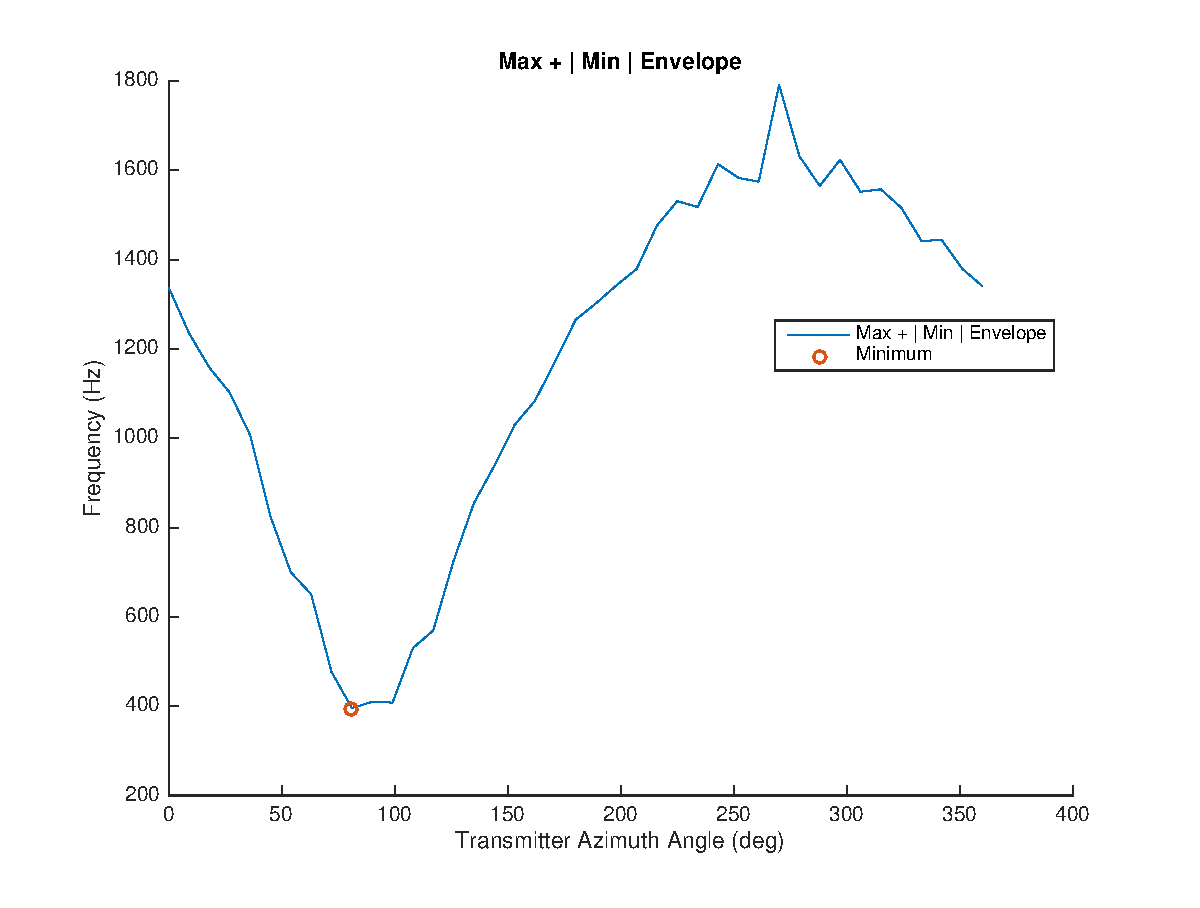
\includegraphics[width=\textwidth]{images/results/Azimuth_angle_estimation_max_plus_absMin_26deg.eps}
        \caption{Elevation Angle of 26.56\textdegree}
         \label{fig:azimuth_estimation_max_plus_absMin_26.56deg}
    \end{subfigure}
    \begin{subfigure}[b]{0.45\textwidth}
        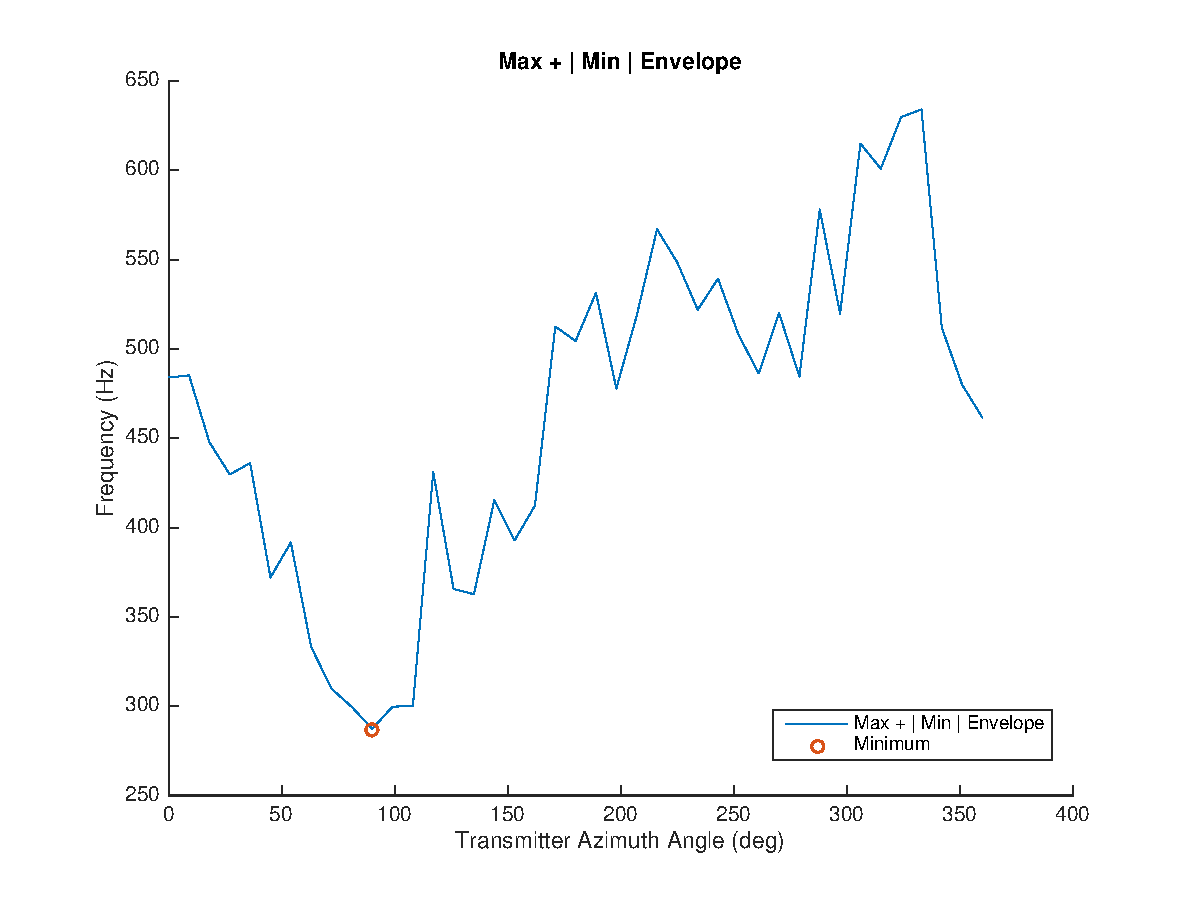
\includegraphics[width=\linewidth]{images/results/Azimuth_angle_estimation_max_plus_absMin_76deg.eps}
        \caption{Elevation Angle of 76\textdegree}
        \label{fig:azimuth_estimation_max_plus_absMin_76deg}
    \end{subfigure}
    \caption{Max plus Absolute value of Min envelope Frequencies vs Transmitter Azimuth Angle}
    \label{fig:two_azimuth_estimation_max_plus_absMin}
 \end{figure}

The error in the estimation for both elevation angles of 45\textdegree \space and 76\textdegree \space are exact matches with no error but at an elevation of 26.56\textdegree \space has an error of 9\textdegree. The issue with this data is that there is a limited sample set of 41 samples around the azimuth range of 360\textdegree. In order to improve the estimation we can combine the information from figure \ref{fig:azimuth_estimation_difference}, which is zero at both azimuth angles of 90\textdegree \space and 270\textdegree, and figure \ref{fig:azimuth_estimation_max_plus_absMin} which contains a global minimum close to 90\textdegree. By taking the absolute value of equation \ref{eqn:difference} and adding that to equation \ref{eqn:addition} we produce equation \ref{eqn:amplified_minimum}

\begin{multline}
	 Amplified Minimum = | Max Upper Envelope - | Min Lower Envelope | | + \\ (Max Upper Envelope + | Min Lower Envelope |)
	 \label{eqn:amplified_minimum}
\end{multline}


figure \ref{fig:amplified_azimuth_estimation} which shows a sharp global minimum at 90\textdegree \space and a sharp local minimum at 270\textdegree alowing for better estimation of the transmitter angle.

  \begin{figure}
	\begin{center}
		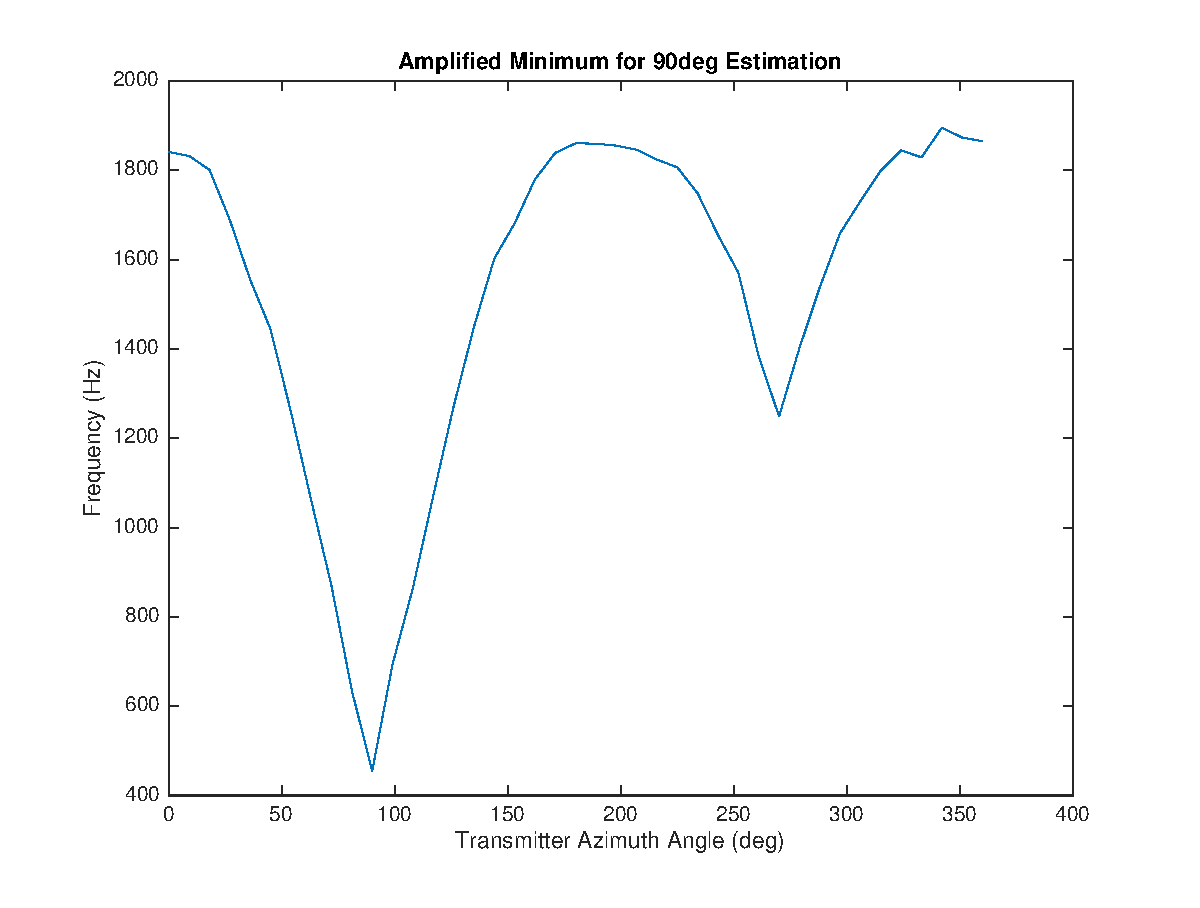
\includegraphics[width=10cm]{images/results/Amplified_azimuth_angle_estimation_45deg.eps}
		\caption{ (-) at an Elevation Angle of 45\textdegree}
		\label{fig:amplified_azimuth_estimation}
	\end{center}
\end{figure}

The error in estimation is zero across all three elevation angles using the $AmplifiedMinimum$ data to find the 90\textdegree azimuth angle by exploiting the fact that the intersections of the two data sets in figure \ref{fig:azimuth_estimation_max_vs_absMin} occur at different frequencies, 90\textdegree \space azimuth intersection at the lower frequency and 270\textdegree \space at a higher frequency.

%-----------------------------------------------------------------------------------------------------------------------------------------------------------------------

\section{Transmitter Elevation Angle Estimation}
%formulate the estimation equation and discuss ambiguity considerations
Using the information gathered from the azimuth estimation procedure we can compute the elevation angle of the transmitter. In the process of gathering azimuth information the maximum and minimum envelopes follow a sinusoidal pattern that contains a maximum doppler information at approximately 180\textdegree \space and 0\textdegree \space azimuth angles. Using that maximum value and the assumption that it comes from a reflection close to the end of the blade we have enough information to determine the elevation angle. 

%using acos to determine angle
The equation from (-) shows how doppler is related to the elevation angle $\alpha$, by assuming that doppler value is coming from the tip of the rotor blade we can solve for $\alpha$

%alpha equation elevation angle
 (theta elevation equation)

%equation for  max doppler on blade at end
(equation max doppler at blade end)

%refer back to elevation angle section in simulations for 180 deg.
Taking the data gathered during the elevation angle simulations in section(-) we can measure the accuracy of the estimation. Figure (-) shows the elevation angle estimation versus the actual, and the percent error of the estimation.

%figure of 180deg estimation and percent error





